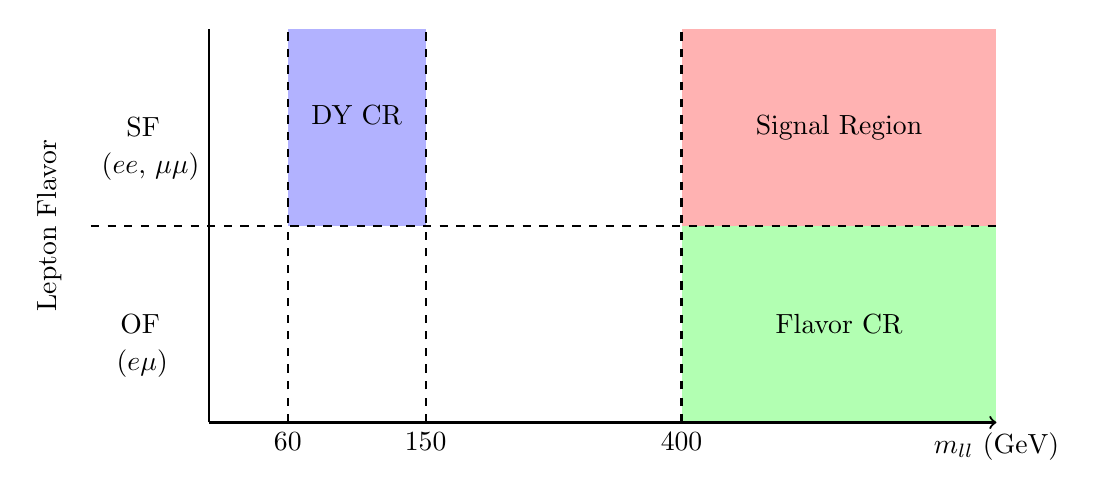
\begin{tikzpicture}[scale=5]
  
    % Define the division points for the vertical regions
    \def\xzero{0.2}   % New left margin division (empty or used for spacing)
    \def\xone{0.55}   % Right boundary of region 1 (DYCR)
    \def\xtwo{1.2}   % Right boundary of region 2 (CR)/left boundary of region 3 (SB)
    \def\xmax{2}      % Overall width of the box

    % -- Fill each grid cell with distinct colors --
    % Column 1: between xzero and xone
    \fill [blue!30!white]    (\xzero,0.5) rectangle (\xone,1);   % Top cell
    \fill [white]    (\xzero,0) rectangle (\xone,0.5);      % Bottom cell

    % Column 2: between xone and xtwo
    \fill [white]   (\xone,0.5) rectangle (\xtwo,1);       % Top cell
    \fill [white]   (\xone,0) rectangle (\xtwo,0.5);         % Bottom cell

    % Column 3: between xtwo and xmax
    \fill [red!30!white]  (\xtwo,0.5) rectangle (\xmax,1);         % Top cell
    \fill [green!30!white]  (\xtwo,0) rectangle (\xmax,0.5);           % Bottom cell
      
    % -- Draw dashed vertical division lines --
    \draw[dashed,thick] (\xzero,0) -- (\xzero,1);  % New left margin boundary
    \draw[dashed,thick] (\xone,0) -- (\xone,1);
    \draw[dashed,thick] (\xtwo,0) -- (\xtwo,1);
    
    % -- Draw a horizontal dashed line (dividing the rows) --
    \draw[dashed,thick] (-0.3,0.5) -- (\xmax,0.5);
    
    % -- Label the y-axis regions (lepton charges) --
    \draw
      (-0.1,0.75) node[anchor=east] {SF}
      (0,0.65) node[anchor=east] {($ee$, $\mu\mu$)}
      (-0.1,0.25) node[anchor=east] {OF}
      (-0.08,0.15) node[anchor=east] {($e\mu$)};
    
    % -- Label the x-axis tick marks (using the original vertical lines) --
    \draw
      (\xzero,0) node[anchor=north] {60}
      (\xone,0) node[anchor=north] {150}
      (\xtwo,0) node[anchor=north] {400};
    
    % -- Axis description on the left --
    \draw
      (-0.35,0.5) node[rotate=90,anchor=south] {Lepton Flavor};
    
    % -- Draw the x-axis as an arrow along the bottom edge --
    \draw[->, thick] (0,0) -- (\xmax,0) node[anchor=north] {$m_{ll}$ (GeV)};
    
    % -- Optionally draw the y-axis line --
    \draw[thick] (0,0) -- (0,1);

    % -- Add internal region labels --
    % Place the label for the DYCR region at the center of the first (red) column:
    \draw ({(\xzero+\xone)/2},0.78) node {DY CR};
    % Place the label for the CR region in the center of the second (blue) column (here using the bottom half for example):
    \draw ({\xtwo+(\xmax-\xtwo)/2},0.25) node[align=center] {Flavor CR};
    % Place the label for the SB region in the center of the third (green) column (using the top half):
    \draw ({\xtwo+(\xmax-\xtwo)/2},0.75) node[align=center] {Signal Region};
    
\end{tikzpicture}